\documentclass[a4paper, 11pt]{article}

\setcounter{tocdepth}{3}
\setcounter{secnumdepth}{3}

\usepackage{comment} % enables the use of multi-line comments (\ifx \fi) 
\usepackage{lipsum} %This package just generates Lorem Ipsum filler text. 
\usepackage{fullpage} % changes the margin
\usepackage[utf8]{inputenc}
\usepackage{gensymb}
\usepackage{graphicx}
\usepackage{booktabs}% http://ctan.org/pkg/booktabs
\usepackage{makecell}
\usepackage{tabularx}
\usepackage[table]{xcolor}
\usepackage{array}
\usepackage{wrapfig}
\usepackage{subcaption}
\usepackage{csquotes}
\usepackage{lscape}
\usepackage{afterpage}
\usepackage{geometry}
\usepackage{listings}
\usepackage{chngcntr}
\usepackage{multicol}

\counterwithin{figure}{section}

\geometry{a4paper, margin=1in}
\renewcommand{\figurename}{Abb.}
\renewcommand{\tablename}{Tabelle}
\newcommand{\code}[1]{\texttt{#1}}

\renewcommand*{\thead}[1]{\bfseries #1}

\renewcommand{\contentsname}{Inhalt}
\renewcommand{\listfigurename}{Abbildungsverzeichnis}

\lstset{frame=tlrb,
	language=Java,
	captionpos=b,
	aboveskip=3mm,
	belowskip=3mm,
	showstringspaces=false,
	columns=flexible,
	basicstyle={\small\ttfamily},
	numbers=left,
	numberstyle=\tiny\color{gray},
	keywordstyle=\color{blue},
	commentstyle=\color{violet},
	stringstyle=\color{darkgreen},
	breaklines=true,
	breakatwhitespace=true,
	tabsize=3,
	literate=%
	{Ö}{{\"O}}1
	{Ä}{{\"A}}1
	{Ü}{{\"U}}1
	{ß}{{\ss}}1
	{ü}{{\"u}}1
	{ä}{{\"a}}1
	{ö}{{\"o}}1
}

\begin{document}
 
\title{Zusammenfassung ENAPP - HS2018}
\author{Alex Neher}
\maketitle

\tableofcontents
\newpage
\listoffigures
\newpage

\graphicspath{{./Pictures/}}


\section{JavaEE}
JavaEE, oder Jave Enterprise Edition, ist eine Alternative zur bereits bekannten JavaSE, oder Java Standard Edition. \\
Im Gegensatz zu JavaSE, wo Applikationen als Standalone Programme z.B. via .jar Files gestartet werden, werden JavaEE Applikationen auf Applikationsserver deployed, wo sie dann in bestimmten Containern laufen und stets zur Verfügung stehen.

\vspace{10px}

Mit 'Container' meint man spezielle Laufzeitumgebungen auf diesen Applikationsserver, die der JVM bestimmte Funktionen zur Verfügung stellt, wie z.B. ein Datenbankzugriff. Es wird zwischen vier Hauptarten von Container unterschieden:

\begin{itemize}
    \item Applet Container
    \item Application Client-Container
    \item Web-Container / Servlet-Container
    \item EJB-Container
\end{itemize}

Diese Container-Arten beinhalten meist die 'passenden' Anwendungs-Komponenten:

\begin{description}
    \item[Applet: ] GUI-Anwendungen im Browser (Eher veraltet heutzutage)
    \item[Application Client: ] Standalone GUI-Applikationen auf dem Client (z.B. als SWING-Applikation)
    \item[JSP / Servlet: ] Web-Komponenten
    \item[EJB: ] Beinhaltet Geschäftslogik einer Umgebung
\end{description}


\begin{figure}[htb]
    \centering
    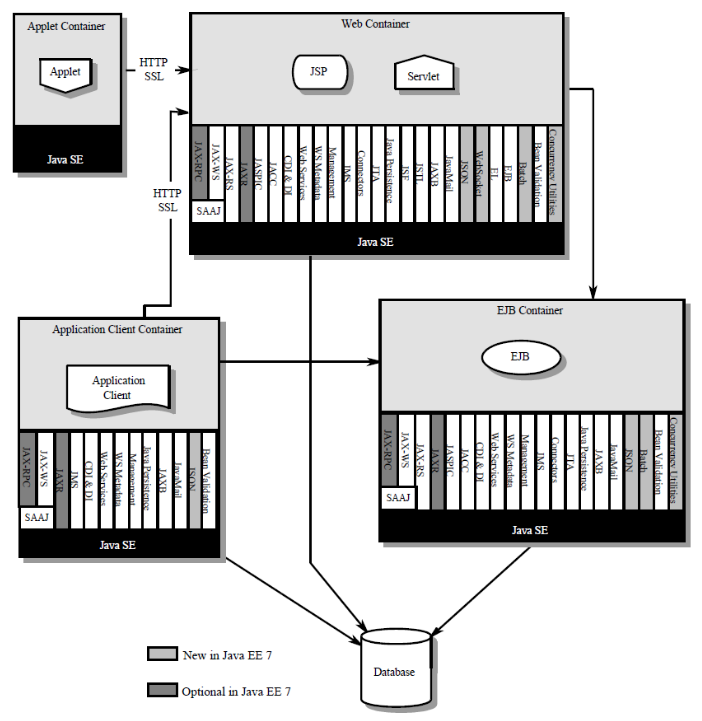
\includegraphics[keepaspectratio=true,height=20\baselineskip]{container_types.png}
    \caption{Verschiedene Container- und Anwendungs-Typen}
    \label{fig:container_types}
\end{figure}

Applikationsserver können entwerder als Full-Profile oder aber als Web-Profile installiert werden. Das Full-Profile enthält alle Container- und Anwendungs-Typen, während das Web-Profil zwar leichter ist, aber auch weniger Funktionen bereitstellt, sondern nur diese, die bei einfacheren Infrastrukturen benötigt werden (so ist z.B. JMS nicht inbegriffen im Web-Profile, da es normalerweise erst bei komplexeren Infrastrukturen benötigt wird)


\section{High Availability (JGroups)}

\section{Web-Tier}
\subsection{Tiers und Architekturen}
Wie bereits in anderen Modulen besprochen wurden, kann eine Applikation in verschiedene \textit{Tiers} unterteilt werden. Normalerweise hat man 2- oder 3-Tier Applikationen, aber theoretisch könnte man so viele Tiers haben wie man will.

\vspace{10px}

Bei 3-Tier Architekturen unterscheidet man zwischen Front-End, Middleware und Back-End, oder \textit{Web Tier, App Tier, DB-Tier}

\begin{figure}[htb]
	\centering
	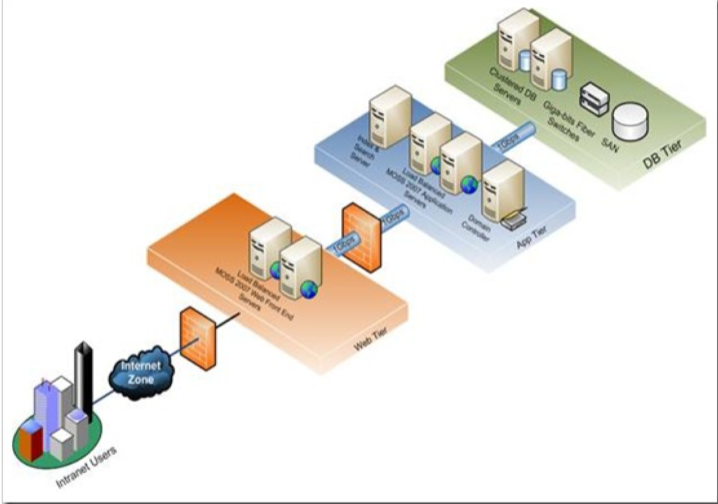
\includegraphics[keepaspectratio=true,height=15\baselineskip]{3-tier.png}
	\caption{Typische 3-Tier Architektur}
	\label{fig:3-tier}
\end{figure}

Alternativ kann auch eine \textit{Web-zentrische Architektur} verwendet werden, bei welcher der Web- und App-Tier konsolidiert werden:

\begin{figure}[htb]
	\centering
	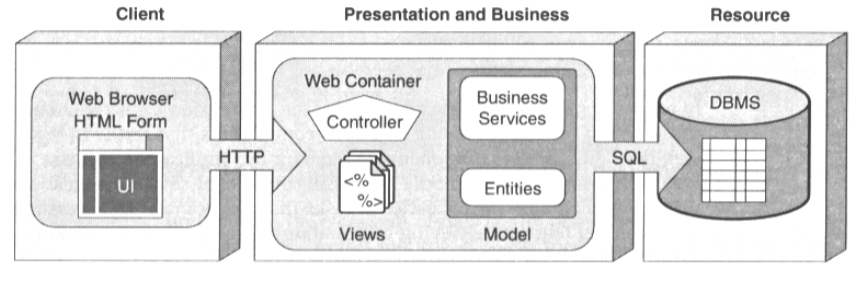
\includegraphics[keepaspectratio=true,height=7.5\baselineskip]{2-tier.png}
	\caption{Das Frontend und die Middleware werden zusammengefasst zu einem einzigen Tier}
	\label{fig:2-tier}
\end{figure}

Wiederum eine weitere Möglichkeit bietet die \textit{B2B-Architektur}. Diese verwendet zwei EJB-Server, die je einen Web- und einen EJB-Container haben. Diese beiden Server können untereinander kommunizieren, meist via REST oder SOAP.

\begin{figure}[htb]
	\centering
	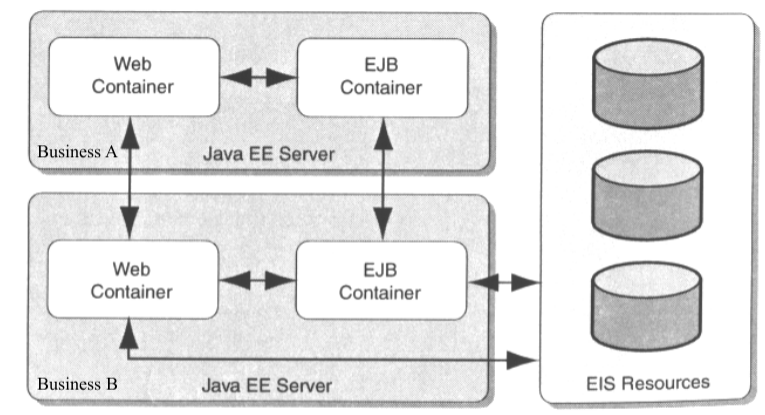
\includegraphics[keepaspectratio=true,height=15\baselineskip]{b2b.png}
	\caption{B2B-Architektur}
	\label{fig:b2b}
\end{figure}

Last but not Least kann auch eine \textit{Web Service Architektur} verwendet werden, wo ein EJB-Container gewisse Funktionen veröffentlicht und eine Stateless Service Bean dient als Zugriffspunkt, die diese veröffentlichte Funktion schliesslich ausführt. Diese Architekturen verwenden meist Messaging.

\begin{figure}[htb]
	\centering
	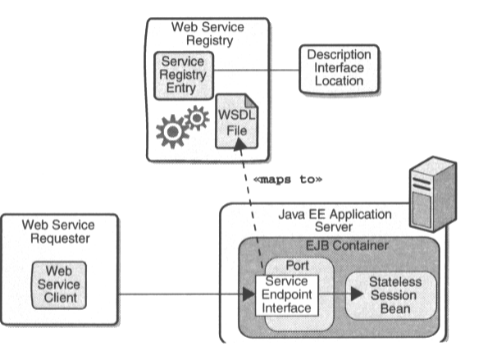
\includegraphics[keepaspectratio=true,height=15\baselineskip]{web-service.png}
	\caption{Web Service Architektur}
	\label{fig:webService}
\end{figure}



\subsection{Komponenten-basiertes Entwickeln}
Diese Art von Entwickeln basiert auf dem Motto \textit{Warum das Rad neu erfinden, wenn man es auch einfach einbinden kann?}. 

\vspace{10px}

JavaEE unterstützt die Verwendung von Komponenten. Komponenten sind eigenständige Software-Elemente, die 'as-is' eingebunden werden können. Das heisst, sie können ohne Änderungen mit anderen eingebunden Komponenten verknüpft und ausgeführt werden.

In der Webshop Applikation wurde zum Beispiel die Komponente des EntityManagers verwendet, um nicht eine ganze Datenbankanbindung in Java programmieren zu müssen. Jeder Programmierer kann jedoch auch seine eigenen Komponenten schreiben. So sind alle Servlets eigene Komponenten, auf welche über die extrahierten Interfaces zugegriffen werden kann.

\vspace{10px}

Komponenten-basiertes Entwickeln bietet einige Vorteile:

\begin{itemize}
	\item  Wiederverwendung von Komponenten
	\item  Austausch von Komponenten
	\item  Lose Kopplung
	\item  Getrennte Entwicklung möglich
	\item  Bessere / gezielte Skalierung
	\item  Verschiedene Sprachen
	\item  Verschiedene Environments
\end{itemize}

\vspace{10px}



Komponenten werden durch \textit{Interfaces} kontrolliert und kommunizieren nicht direkt miteinander. Die Methoden werden ausschliesslich über die Interfaces aufgerufen.

\subsection{MVC}

\begin{wrapfigure}[12]{R}{0.5\textwidth}
	\centering
	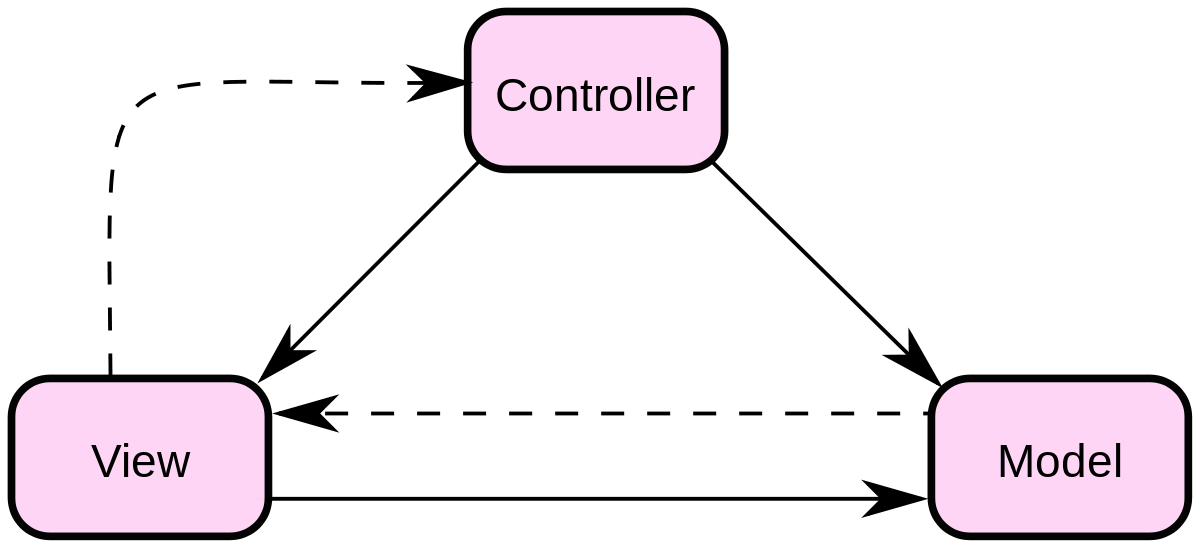
\includegraphics[keepaspectratio=true,height=7.5\baselineskip]{mvc.png}
	\caption{MVC}
	\label{fig:mvc}
\end{wrapfigure}

MVC steht \textit{Model View Control} und ist eine Design-Pattern, die beschreibt, wie eine Applikation aufgebaut ist. 

MVC basiert auf dem Komponenten-basierten Entwickeln und besagt, dass Model (Daten), Control (Logik) und View (Präsentation) voneinander getrennt sein sollten ($\rightarrow$ 3-Tier Architektur (Abb. \ref{fig:3-tier})) und jede Komponente bei Bedarf ausgetauscht werden können sollte ohne die anderen beiden zu beeinträchtigen.

\begin{description}
	\item[Model: ] \textit{Daten Logik}
	\begin{itemize}
		\item Datenbank-Anbindung (oder sonstige Daten, wie z.B. JSON-File) mit CRUD-Funktionalitäten
		\item Kommuniziert mit mit dem Controller - Controller requested Daten und Model liefert sie
		\item Je nach dem kann Model auch View direkt mit neuen Daten updaten
	\end{itemize}
	\item[View: ] \textit{Front-End}
	\begin{itemize}
		\item Was der End-User tatsächlich sieht (z.B. HTML/CSS Frontend bei Web-Apps)
		\item Kommuniziert mit dem Controller, der Daten zur Verfügung - z.B. über dynamische Variablen (siehe JSF mit Servlets oder Angular)
	\end{itemize}
	\item[Controller] \textit{Logik}
	\begin{itemize}
		\item Verarbeitet User-Input von der View
		\item Requestet verlangte Daten vom Model und verarbeitet sie
		\item Übergibt Daten der View
	\end{itemize}

\end{description}

\subsection{Thread Safety}
Aufgrund dessen, dass Java Multithreading unterstützt, müssen (oder sollten) gewisse Vorsichtsmassnahmen getroffen werden, um Datenkorruption oder Programm-Crashes zu verhindern. \\
Die wichtigsten Sicherheitsvorkehrungen:

\begin{description}
	\item[Instanzvariablen: ] Instanzvariablen sollten so private wie möglich behalten werden (optimalerweise \textit{local} und/oder \textit{final}) um den Zugriff von anderen Threads zu erschweren oder zu verunmöglichen
	\item[Klassenvariablen: ] Möglichst keine Klassenvariablen verwenden. Auch wenn \texttt{synchronized} verwendet wird, kann man nicht darauf gehen, dass nicht andere Methoden auch auf diese Variable zugreifen (z.B. via \texttt{getter- } und \texttt{setter-} Methoden)
	\item[Ressourcen-Zugriff: ] Aufpassen bei der Vergabe von Zugriff auf externe Ressourcen. So ist der Zugriff auf das Filesystem sehr kritisch bei mehreren Threads und kann zu korrupten Dateien führen.
	\item[\texttt{synchronized}] Bei kritischen Codestellen sollte zwingend die \texttt{synchronized}-Methode verwendet werden:
	
	\begin{lstlisting}
	synchronized(this){
		//kritischer Code - Hier ist immer nur ein Thread auf einmal
	}
	\end{lstlisting}
\end{description}

\subsection{Servlet Programmieren}
Ein Servlet besteht aus drei Komponenten:

\begin{description}
	\item[label] description
\end{description}

\subsection{Server Domain Mappings und Filter}


\section{EJB-Tier}

EJB steht für "Enterprise Java Bean". Sie sind serverseitige Komponenten, die die Business-Logik einer Applikation zusammenfassen. Sie  stellen Services wie z.B. Transationen, Logging oder Security zur Verfügung. \\
Grundsätzlich wird zwischen vier Arten von Beans unterschieden:

\subsection{Typen von EJBs}
\begin{description}
    \item[@Stateless: ] Stellen zustandlose Dienste zur Verfügung (Jede Anfrage wird als neue Anfrage behandelt, es wird nichts zwischengespeichert)
    \item[@Stateful: ] Stellen zustandsbehaftete Dienste zur Verfügung (Es werden gewisse Informationen zwischengespeichert, die bei späteren Anfragen wiederverwendet werden können)
    \item[@Singleton: ] Existiert genau einmal in der gesamten Applikation und stellt einen zustandsbehafteten Service zur Verfügung
    \item[@MessageDriven: ] Reagieren auf asynchrone Messages
\end{description}

Diese Beans sind nicht automatisch von überall her sichtbar und können auch nicht von überall her benutzt werden. Es muss eine Sichtbarkeit festgelegt werden:

\begin{description}
    \item[@Local: ] Von allen Komponenten innerhalb derselben JVM sichtbar (Es können mehrere Applikationen auf einem Applikationsserver laufen. Diese können nun alle auf diese Bean zugreifen)
    \item[@Remote: ] Auch für Anwendungen sichtbar, die ausserhalbe der JVM laufen
    \item[@LocalBean: ] Nur innerhalb des EAR-Projekts der Applikation sichtbar, also ausschliesslich innerhalb dieser Applikation
\end{description}
Typen von EJBs


\subsection{Dependency Injection}

Anstelle, dass ich zum Beispiel mühsam eine Datenbank-Anbindung mit Java implementiere, kann ich die auch einfach einbinden, da sich jemand anders schon die Mühe gemacht hat, das Ding zu schreiben. Einen solchen \texttt{PersistenceContext} kann ich mit zwei Zeilen Code einbinden:

\begin{lstlisting}
@PersistenceContext
private EntityManager em;
\end{lstlisting}

Wenn ich nun etwas in die Datenbank speichern will, kann ich auf eine Methode dieses EntityManagers zugreifen

\begin{lstlisting}
em.persist(Object object);
\end{lstlisting}

\section{JEE Security}

\section{Messaging Services}

\section{REST}

\section{JNDI \& LDAP}

\section{CDI}

\section{Architektur \& Agiles Vorgehen}

\end{document}
